
\begin{flushleft}
	
	A Java identifier is a name of a variable, function, class, module or other object.
	\newline
	Eg:
	\begin{tcolorbox}[breakable,notitle,boxrule=-0pt,colback=code,colframe=code]
		\color{black}
		\fontdimen2\font=8pt
		package \textbf{Starter}; \newline
		\newline
		public class \textbf{Test} \{ \newline
		\hphantom{} \hphantom{}	public static void main(\textbf{String}[] \textbf{args}) \{ \newline
		\hphantom{} \hphantom{} \hphantom{} \hphantom{}	int \textbf{x}=999; \newline
		\hphantom{} \hphantom{} \hphantom{} \hphantom{}	System.out.println(x); \newline
		\hphantom{} \hphantom{}	\} \newline
		\}
		\fontdimen2\font=4pt
	\end{tcolorbox}
	
	\bigskip
	In above code, there are total 6 identifiers:
	\begin{itemize}
		\item Starter - name of package
		\item Test - name of class
		\item main - name of function
		\item String - name of class 
		\item args - name of object
		\item x - name of integer variable
	\end{itemize}
	
	\textbf{Rules of identifiers:}
	\begin{itemize}
		\item Names can contain A-Z, a-z, 0-9, \_, and \$ signs.
		\item Names cannot begin with number.
		\item Names are case sensitive ("myVar" and "myvar" are different variables).
		\item Reserved words (like Java keywords, such as int or boolean) cannot be used as names.
		\item Names can be of any length, but it's not recommended to have big names.
		\item Developers should declare identifiers using the \textbf{Camel case} writing style (e.g., StringBuilder, isAdult)
	\end{itemize}
	
	\bigskip
	\begin{figure}[h!]
		\centering
		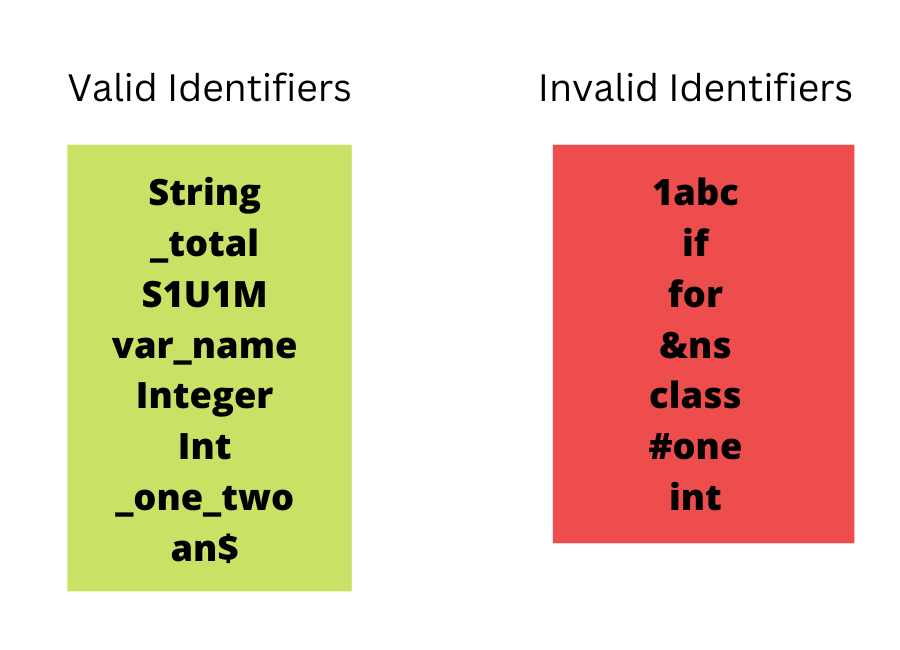
\includegraphics[scale=.45]{content/chapter2/images/java.png}
	\end{figure}
	
	
\end{flushleft}


